\documentclass[10pt,a4paper]{article}
\usepackage[utf8]{inputenc}
\usepackage[portuguese]{babel}
\usepackage[T1]{fontenc}
\usepackage{amsmath}
\usepackage{mathtools}
\usepackage{amsfonts}
\usepackage{amssymb}
\usepackage{graphicx}
\usepackage[left=2.5cm,right=2.5cm,top=2.5cm,bottom=2.5cm]{geometry}
\usepackage{listings}
\usepackage{color} %red, green, blue, yellow, cyan, magenta, black, white
\definecolor{mygreen}{RGB}{28,172,0} % color values Red, Green, Blue
\definecolor{mylilas}{RGB}{170,55,241}

\newcommand{\prt}[1]{\left(#1\right)}
\newcommand{\col}[1]{\left[#1\right]}
\newcommand{\chv}[1]{\left\{#1\right\}}
\newcommand{\hgf}[4]{\prescript{}{2}{F}_1\left(#1,#2,#3,#4\right)}

\author{Murilo Camargos}
\title{Métodos Computacionais - Aula 4}
\begin{document}
\lstset{extendedchars=true, inputencoding=latin1,literate=
{á}{{\'a}}1
{à}{{\`a}}1
{ã}{{\~a}}1
{é}{{\'e}}1
{ê}{{\^e}}1
{í}{{\'i}}1
{ó}{{\'o}}1
{õ}{{\~o}}1
{ú}{{\'u}}1
{ü}{{\"u}}1
{ç}{{\c{c}}}1}
\lstset{language=Matlab,%
    %basicstyle=\color{red},
    breaklines=true,%
    morekeywords={matlab2tikz},
    keywordstyle=\color{blue},%
    morekeywords=[2]{1}, keywordstyle=[2]{\color{black}},
    identifierstyle=\color{black},%
    stringstyle=\color{mylilas},
    commentstyle=\color{mygreen},%
    showstringspaces=false,%without this there will be a symbol in the places where there is a space
    numbers=left,%
    numberstyle={\tiny \color{black}},% size of the numbers
    numbersep=9pt, % this defines how far the numbers are from the text
    emph=[1]{for,end,break},emphstyle=[1]\color{red}, %some words to emphasise
    %emph=[2]{word1,word2}, emphstyle=[2]{style},
    extendedchars=true,
    inputencoding=latin1, 
}


	\section{(Nossa versão da) Equação de Rayleigh-Plesset (24/11/2017)}
	
	A equação mais geral do raio da bolha ao longo do tempo é
	
	\begin{equation}
	\begin{split}
	\partial_t\prt{\prt{I_1+I_2}\prt{R(t)}^3R'(t)} = \prt{2I_2-I_1}\prt{R(t)}^2\prt{R'(t)}^2 + \Lambda\\ - \int_0^{R(t)}{r^2T'\prt{R(t)}\partial_{T(R(t))}\epsilon\prt{n,T(R(t))}dr}\\ - \int_{R(t)}^\infty{r^2T'\prt{R(t)}\partial_{T(R(t))}\epsilon\prt{n,T(R(t))}dr}
	\end{split}
	\end{equation}
	
	em que $T$ é uma temperatura, $\epsilon$ uma energia e
	
	\[I_1 = \int_0^1{\frac{x^4F(x)}{1-x^2(R'(t))^2}dx}, \hspace{1cm} I_2 = \int_1^\infty{\frac{x^2F(x)}{x^4-(R'(t))^2}dx}\]
	\[\Lambda = \int_0^{R(t)}{\frac{3r^2F(r)}{R(t)}dr} - \prt{R(t)}^2\chv{F(r\rightarrow\infty) + \epsilon_v\col{n(r\rightarrow R), T\prt{R(t)}} - \epsilon_l\col{n(r\rightarrow R), T(R(t))}}\]
	
	Para um campo termodinâmico espacialmente uniforma, $F=F_0$ e as I-integrais tornam-se:
	\[I_1 = \frac{1}{5}F_{0,v}\cdot\hgf{1}{\frac{5}{2}}{\frac{7}{2}}{\prt{R'(t)}^2}\]
	\[I_2 = F_{0,l}\cdot\hgf{1}{\frac{1}{4}}{\frac{5}{4}}{\prt{R'(t)}^2}\]
	
	em que a função hipergeométrica $\prescript{}{2}{F}_1$ é conhecida por admitir a representação integral
	\[\hgf{a}{b}{c}{z} = \frac{\Gamma(c)}{\Gamma(b)\Gamma(c-b)}\int_0^1{\frac{\zeta^{b-1}\prt{1-\zeta}^{-b+c-1}}{\prt{1-\zeta z}^a}d\zeta}\]
	
	No caso da teoria de uma temperatura zero, a equação da bolha por ser escrita na forma
	\[R''(t) = \frac{\Lambda-\prt{R(t)}^2\prt{4I_1(t)+I_2(t)}\prt{R'(t)}^2-\prt{R(t)}^3R'(t)\prt{I_1'(t)+I_2'(t)}}{\prt{R(t)}^3\prt{I_1(t)+I_2(t)}}\]
	
	Se os componentes do líquido e do vapor são homogêneos, temos:
	\[R''(t) = \frac{35\Lambda + \prt{R(t)}^2\prt{-28F_{0,v}H_1-35F_{0,l}H_2}\prt{R'(t)}^2}{\prt{R(t)}^3\chv{F_{0,v}\col{7H_1+10H_3\prt{R'(t)}^2}+7F_{0,l}\col{5H_2+2H_4\prt{R'(t)}^2}}}\]
	
	em que:
	\[H_1 = \hgf{1}{\frac{5}{2}}{\frac{7}{2}}{\prt{R(t)}^2} \hspace{1cm} H_2 = \hgf{1}{\frac{1}{4}}{\frac{5}{4}}{\prt{R(t)}^2}\]
	\[H_3 = \hgf{2}{\frac{7}{2}}{\frac{9}{2}}{\prt{R(t)}^2} \hspace{1cm} H_4 = \hgf{2}{\frac{5}{4}}{\frac{9}{4}}{\prt{R(t)}^2}\]
	\[\Lambda = \prt{R(t)}^2\col{-F(r\rightarrow\infty) + F_{0,v} + \epsilon_l(n(r\rightarrow R),0) - \epsilon_v(n(r\rightarrow R),0)}\]
	
	Neste ponto, lembramos a relação termodinâmica $n\epsilon'(n)=F(r)=P+\epsilon$, conhecida como \textbf{relação de Gibbs}. O primeiro termo do numerador do lado direito da equação pela $R''(t)$ se torna:
	\[35\prt{R(t)}^2\prt{-P_l+P_v}\hspace{2cm}(-P_l+P_v=-beta)\]
	Fazendo as substituições:
	\[F_{0,l}=\epsilon_l+P_l, \hspace{.2cm} F_{0,v}=\epsilon_v+P_v, \hspace{.2cm} H_1=5I_1, \hspace{.2cm} H_2=I_2, \hspace{.2cm} H_3=\frac{7}{2}I_3,\hspace{.2cm}  H_4=\frac{5}{2}I_4,\]
	temos a equação da lista.
	
	\section{Exercícios}
	Use o método de integração de Runge-Kutta para obter a aproximação da solução dos seguintes problemas de Cauchy\\
	
	1. \[R'(t)=U(t), \hspace{0.3cm} U'(t)=-\frac{R'(t)^2\col{I_2\prt{P_l+\epsilon_l} + 4I_1\epsilon_v}+P_l+P_v\prt{4I_1R'(t)^2-1}}{R(t)\col{I_4\prt{P_l+\epsilon_l}R'(t)^2+I_2\prt{P_l+epislon_l}+\prt{P_v+\epsilon_v}\prt{I_1+I_3R'(t)^2}}}\]
	\[R(0)=0.1, \hspace{.3cm} U(0)=0.1\]
	
	2. \[R'(t)=U(t), \hspace{0.3cm} U'(t)=-\frac{R'(t)^2\col{I_2\prt{P_l+\epsilon_l} + 4I_1\epsilon_v}+P_l+P_v\prt{4I_1R'(t)^2-1}}{R(t)\col{I_4\prt{P_l+\epsilon_l}R'(t)^2+I_2\prt{P_l+epislon_l}+\prt{P_v+\epsilon_v}\prt{I_1+I_3R'(t)^2}}}\]
	\[R(0)=0.2, \hspace{.3cm} U(0)=\frac{1}{10000000}\]
	
	Adote os seguintes valores para os parâmetros: $P_v=0.1595106949435665$, $P_l=0.17078553413498362$, $\epsilon_v=1.7699955011416335$ e $\epsilon_l=4.275051939160018$. Note que $U$ é a primeira derivada de $R$ com relação a $t$.
	
	As integrais que aparecem na equação que trata da determinação de $R$ são expressas em termos das funções hipergeométricas:
	\[I_1=\frac{1}{5} \hgf{1}{\frac{5}{2}}{\frac{7}{2}}{\prt{R(t)}^2} = \frac{1}{2}\int_0^1{\frac{\zeta^{3/2}}{1-\zeta R'(t)}d\zeta}\]
	\[I_2=\hgf{1}{\frac{1}{4}}{\frac{5}{4}}{\prt{R(t)}^2} = \frac{1}{4}\int_0^1{\frac{1}{\zeta^{3/4}\prt{1-\zeta R'(t)}}d\zeta}\]
	\[I_3=\frac{2}{7}\hgf{2}{\frac{7}{2}}{\frac{9}{2}}{\prt{R(t)}^2} = \int_0^1{\frac{\zeta^{5/2}}{\prt{1-\zeta R'(t)}^2}d\zeta}\]
	\[I_4=\frac{2}{5}\hgf{2}{\frac{5}{4}}{\frac{9}{4}}{\prt{R(t)}^2} = \frac{1}{2}\int_0^1{\frac{\zeta^{1/4}}{\prt{1-\zeta R'(t)}^2}d\zeta}\]
	
	\newpage
	\section{Resolução}
	Os testes foram feitos no Matlab e foram utilizadas as funções já criadas nos exercícios anteriores.
	\subsection{Exercício 1}
	Na primeira equação, por haver velocidade inicial considerável, o gráfico descreve o formato de uma parábola. Para a resolução desta questão, foi utilizado um passo igual a $0.01$ no Runge-Kutta de quarta ordem e o valor do tempo de colapso (aproximadamente \textbf{6.01}) foi encontrado por tentativa e erro.
	
	\begin{figure}[h!]
    \centering
      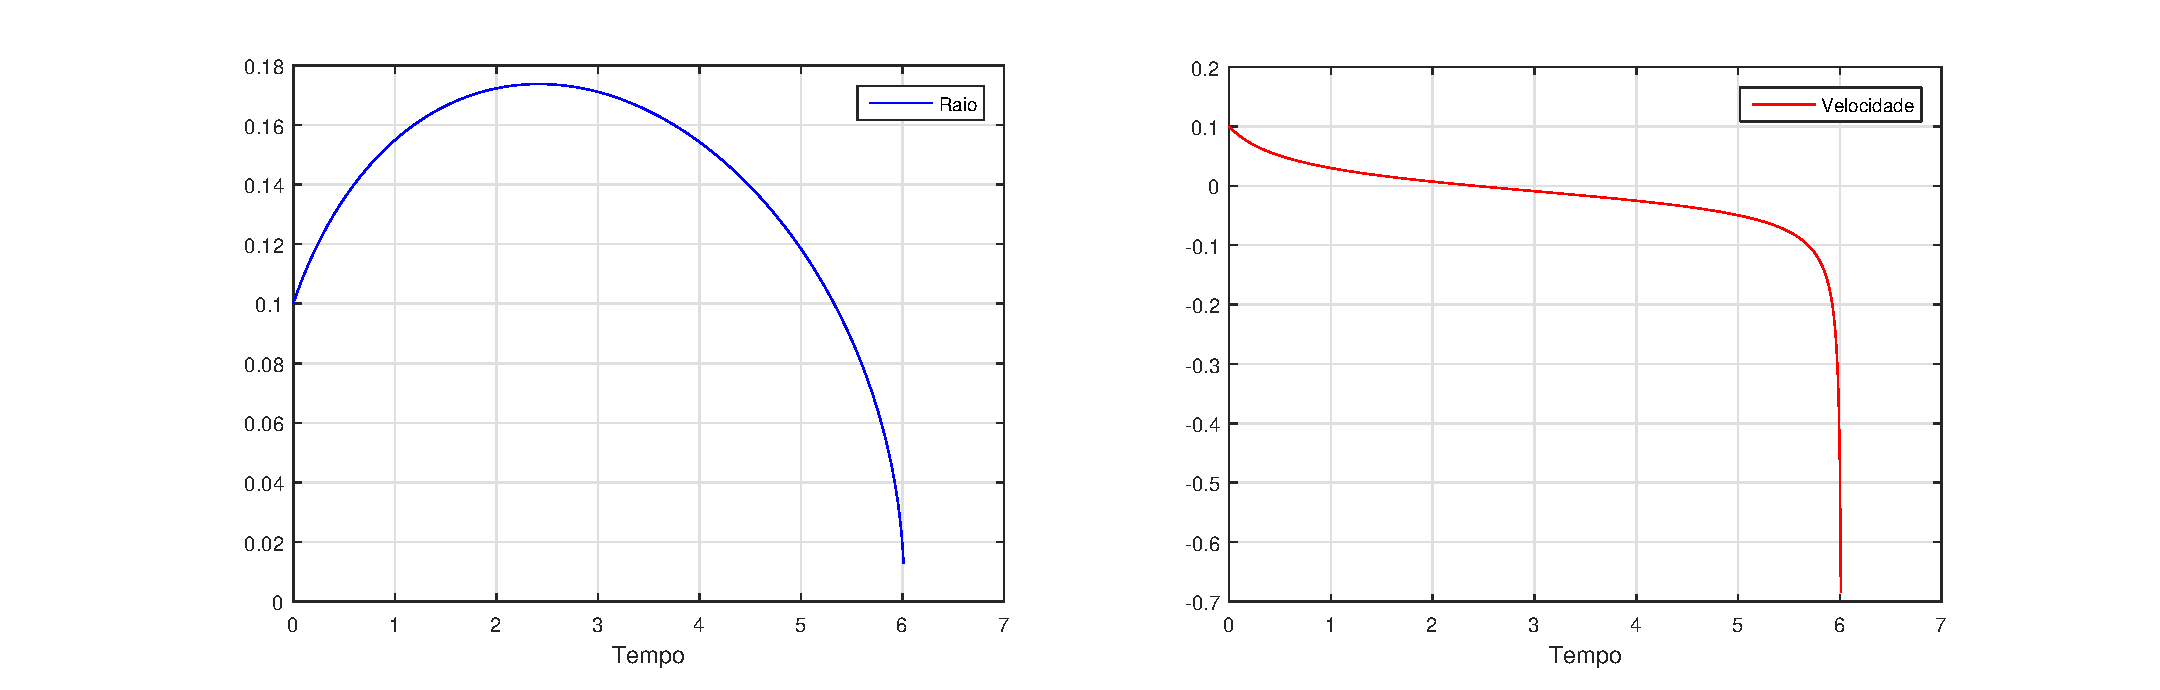
\includegraphics[width=1\linewidth]{figures/eq1-h0-01-t-6-01.eps}
      \caption{Raio e velocidade da bolha ao longo do tempo para o exercício 1.}
      \label{fig:raio1}
	\end{figure}
	
	\subsection{Exercício 2}
	Para a segunda equação, foi utilizado um passo também igual a $0.01$ no Runge-Kutta de quarta ordem e o valor do tempo de colapso (aproximadamente \textbf{4.14}) foi encontrado por tentativa e erro.
	
	\begin{figure}[h!]
    \centering
      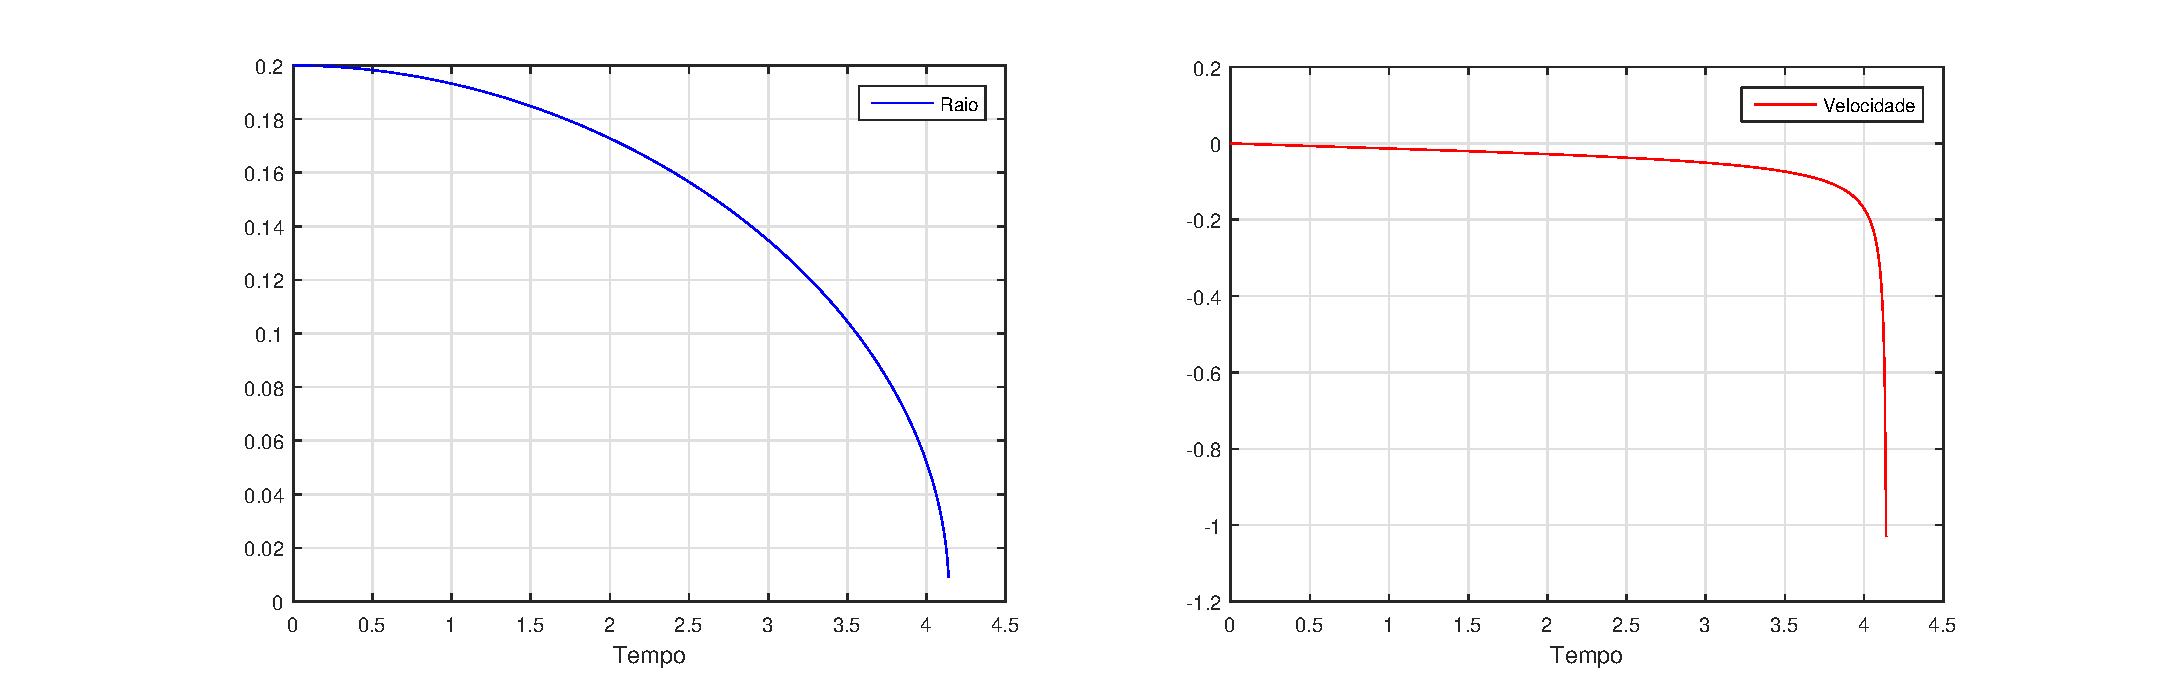
\includegraphics[width=1\linewidth]{figures/eq2-h0-01-t-4-14.eps}
      \caption{Raio e velocidade da bolha ao longo do tempo para o exercício 2.}
      \label{fig:raio2}
	\end{figure}
    
    \newpage
    \subsection{Código em MATLAB}
    \lstinputlisting[language=matlab]{code/bolha_geral.m}
    \subsection{Código da função hipergeométrica 2F1}
    \lstinputlisting[language=matlab]{../tools/hg2F1.m}
	
\end{document}